\section{Câu d: Data Preparation}
\label{sec:d}

Đầu vào là dữ liệu đã xử lý và đóng băng ở câu c (script kiểm tra mã băm trước khi chạy). Mục tiêu là một ma trận số cho thuật toán dựa trên khoảng cách, trong đó mỗi thuộc tính đóng góp một cách có chủ đích.

\subsection{Chuẩn hóa: so sánh StandardScaler, MinMaxScaler và RobustScaler}
Ba bộ chuẩn hóa khác nhau ở thứ được dùng để đặt thang: trung bình và độ lệch chuẩn (Standard), min và max (MinMax), trung vị và IQR (Robust). Với phân cụm dựa trên khoảng cách, điều quan trọng là mỗi cột đóng góp ngang nhau và vài dòng không chi phối.
Trên 10 cột số của dữ liệu đã xử lý (Bảng~\ref{tab:scaler}):
\begin{itemize}
\item \textbf{Standard} làm mỗi cột có phương sai 1 (đúng giả định cân bằng của K-Means) nhưng nhạy với cực trị khi dữ liệu chưa log (17 ô vượt $4$ độ lệch chuẩn).
\item \textbf{MinMax} đặt thang theo min/max nên một cực trị quyết định thang cả cột; vì ta giữ các cực trị hợp lệ, phần lớn khách bị nén vào một đoạn hẹp (cột lớn nhất chiếm 24,7--30,7\% phương sai).
\item \textbf{Robust} bền khi \emph{tính thang} nhưng \emph{không chặn} cực trị: trên dữ liệu thô một khách ``cá voi'' nằm cách 85 đơn vị IQR và 5 dòng chiếm 80,7\% tổng bình phương, nên Robust chỉ phù hợp sau khi đã log.
\end{itemize}
Chọn \textbf{log1p + StandardScaler}: cân bằng nhất (cột lớn nhất 11,9\%, gần $1/10$) và ít bị vài dòng chi phối nhất trong nhóm cột có phương sai bằng nhau. Robust sau log là phương án gần tương đương (không lưu riêng).

\begin{table}[htbp]
\centering\small
\caption{So sánh bộ chuẩn hóa trên 10 cột số (thô hoặc sau log1p). ``5 dòng'' là phần tổng bình phương độ lệch do 5 dòng lớn nhất nắm giữ; ``cột lớn nhất'' là phần phương sai của cột lớn nhất.}
\label{tab:scaler}
\begin{tabular}{lcccc}
\toprule
Biểu diễn & 5 dòng & Cột lớn nhất & $\max|\text{giá trị}|$ & Ô vượt $4$ sd\\
\midrule
thô + Standard & 21,9\% & 11,3\% & 12,7 & 17\\
thô + MinMax & 7,7\% & 30,7\% & 1,0 & 17\\
thô + Robust & 80,7\% & 52,3\% & 85,2 & 17\\
log1p + \textbf{Standard} & \textbf{6,6\%} & \textbf{11,9\%} & 5,8 & 2\\
log1p + MinMax & 4,6\% & 24,7\% & 1,0 & 2\\
log1p + Robust & 8,8\% & 16,9\% & 5,5 & 2\\
\bottomrule
\end{tabular}
\end{table}

\subsection{Mã hóa biến phân loại và vấn đề one-hot chi phối khoảng cách}
Biến thứ tự \var{membership_tier} được mã $0/1/2$ rồi z-score (giữ thứ tự bronze $<$ silver $<$ gold, một cột); biến nhị phân \var{app_installed} chỉ z-score.
Biến định danh \var{device_type} (3 mức) và \var{preferred_category} (5 mức) dùng one-hot. Nếu z-score luôn các cột dummy thì mức hiếm bị khuếch đại: dummy \texttt{unknown} (5\% dòng) có $z=4{,}36$ và khối \var{preferred_category} chiếm 30\% tổng phương sai
dù chỉ là một biến trên 13. Nếu để dummy 0/1 thô thì mỗi biến định danh đóng góp ít hơn một cột số. Giải pháp: giữ dummy 0/1 và nhân với trọng số $w$ sao cho \emph{kỳ vọng bình phương khoảng cách giữa hai khách ngẫu nhiên} của biến đó bằng với một cột số chuẩn hóa.

Với biến định danh có xác suất các mức $p_j$, hai khách khác mức có khoảng cách bình phương $2w^2$ và cùng mức có khoảng cách $0$, nên
\begin{equation}
\mathbb E[d^2] = 2w^2\Big(1-\sum_j p_j^2\Big) \overset{!}{=} 2 \quad\Longrightarrow\quad w = \frac{1}{\sqrt{1-\sum_j p_j^2}} .
\end{equation}
Vế phải $2$ là kỳ vọng $\mathbb E[(z_i-z_j)^2]=2\,\mathrm{Var}(z)$ của một cột z-score. Kết quả: $w_{\mathrm{device}}=1{,}301$, $w_{\mathrm{category}}=1{,}125$ (tính trên 247 nhãn đã biết). Mức \texttt{unknown} được mã bằng hàng toàn số $0$ ở khối category,
tức cách đều mọi nhãn và không tạo trục riêng cho 13 dòng.

\begin{table}[htbp]
\centering\small
\caption{Tỉ trọng phương sai theo khối trong ma trận thiết kế với ba cách mã hóa. Mỗi biến số/hạng/nhị phân/device của mã hóa C đóng góp đúng 7,71\% khoảng cách (category 7,43\%).}
\label{tab:blocks}
\begin{tabular}{lcccc}
\toprule
Mã hóa & Số (9 cột) & Hạng + nhị phân & \var{device_type} & \var{preferred_category}\\
\midrule
A. z-score cả dummy & 45,0\% & 10,0\% & 15,0\% & \textbf{30,0\%}\\
B. dummy 0/1 thô & 72,9\% & 16,2\% & 4,8\% & 6,2\%\\
C. dummy $\times\,w$ (chính) & 69,4\% & 15,4\% & 7,7\% & 7,4\%\\
\bottomrule
\end{tabular}
\end{table}

\subsection{Chọn thuộc tính, giảm chiều và thuật toán}
\paragraph{Thuộc tính dư thừa.} Trên thang log, $R^2$ của $\ln$(\var{total_spend_12m}) theo $\ln$(\var{n_orders_12m}) và $\ln$(\var{avg_order_value}) là $0{,}987$ (VIF $82{,}5$): \var{total_spend_12m} gần như là hàm của hai cột kia theo định nghĩa.
Bỏ nó làm VIF của \var{n_orders_12m} giảm từ $67{,}1$ xuống $7{,}3$ và của \var{avg_order_value} từ $14{,}8$ xuống $2{,}3$. Các cột khác có $R^2\le 0{,}90$ và ý nghĩa nghiệp vụ riêng (ví dụ \var{pages_per_session} VIF $10{,}2$) nên được giữ.
Phiên bản giữ lại \var{total_spend_12m} được lưu riêng (\var{X_full_features}).

\paragraph{PCA.} Giữ 90\% phương sai cần 9 trong 19 thành phần nhưng chỉ bảo toàn $74\%$ lân cận 5-NN so với không gian đầy đủ (5 thành phần chỉ $55\%$): các hướng phương sai thấp mang thông tin cục bộ.
Với $N=260$ và 19 cột không cần giảm chiều để tính toán, và không giảm chiều chỉ để biểu đồ đẹp hơn; PCA 90\% chỉ là biến thể để so sánh (Hình~\ref{fig:d_red}).

\paragraph{K-Means, K-Prototypes hay Gower.} Dữ liệu hỗn hợp nhưng thiên về số: 9 cột số, 1 hạng, 1 nhị phân, 2 định danh (13 thuộc tính sau chọn lọc), và quan hệ của biến phân loại với biến số yếu
(câu b: Cramér $V\le 0{,}24$; $\varepsilon^2$ của thiết bị $\le 0{,}11$). K-Means trên ma trận trên là phương án chính: với $w$, mỗi biến đóng góp ngang nhau, tức đã làm điều mà tham số $\gamma$ của K-Prototypes phải điều chỉnh,
và $\gamma$ không có giá trị ``đúng'' trong học không giám sát. K-Prototypes không chạy được (môi trường không có thư viện \texttt{kmodes}). Thay vào đó lưu ma trận khoảng cách Gower ($260\times260$, bỏ biến khi \texttt{unknown})
cho phân cụm phân cấp; hình học của nó khác $X_{\text{main}}$ rõ (5-NN trùng $0{,}71$, tương quan hạng khoảng cách $0{,}894$).

\subsection{Kết quả chuẩn bị}
Số thuộc tính: \textbf{14 $\to$ 13 $\to$ 19 cột} (bỏ \var{total_spend_12m}; mã hóa tạo 3 + 5 cột one-hot). Ma trận chính $X_{\text{main}}$ gồm: 6 cột log1p + z-score (\var{n_orders_12m}, \var{avg_order_value}, \var{recency_days}, \var{sessions_per_month}, \var{avg_session_minutes}, \var{pages_per_session}),
3 cột z-score (\var{age}, \var{discount_usage_rate}, \var{cart_abandon_rate}), 1 cột hạng, 1 cột nhị phân, 3 cột dummy device và 5 cột dummy category (nhân $w$); 260 hàng, không NaN/inf, không có \var{customer_id} hay cờ metadata.
Độ lệch (skew) sau biến đổi: \var{n_orders_12m} $3{,}33\to0{,}52$, \var{sessions_per_month} $1{,}16\to-0{,}63$, \var{avg_session_minutes} $2{,}07\to0{,}47$, \var{pages_per_session} $1{,}64\to0{,}52$, \var{recency_days} $1{,}67\to-0{,}55$;
\var{avg_order_value} chỉ giảm từ $10{,}92$ xuống $1{,}67$ và vẫn có $z$ lớn nhất $5{,}8$ vì các cực trị hợp lệ được giữ lại.
Tỉ trọng khoảng cách: trước chuẩn bị (số thô, không scale) \var{total_spend_12m} chiếm 99,78\% và mọi cột còn lại gộp 0,22\%; sau chuẩn bị mỗi biến chiếm $\approx 7{,}7\%$ (Hình~\ref{fig:d_enc}).

\begin{figure}[htbp]
\centering
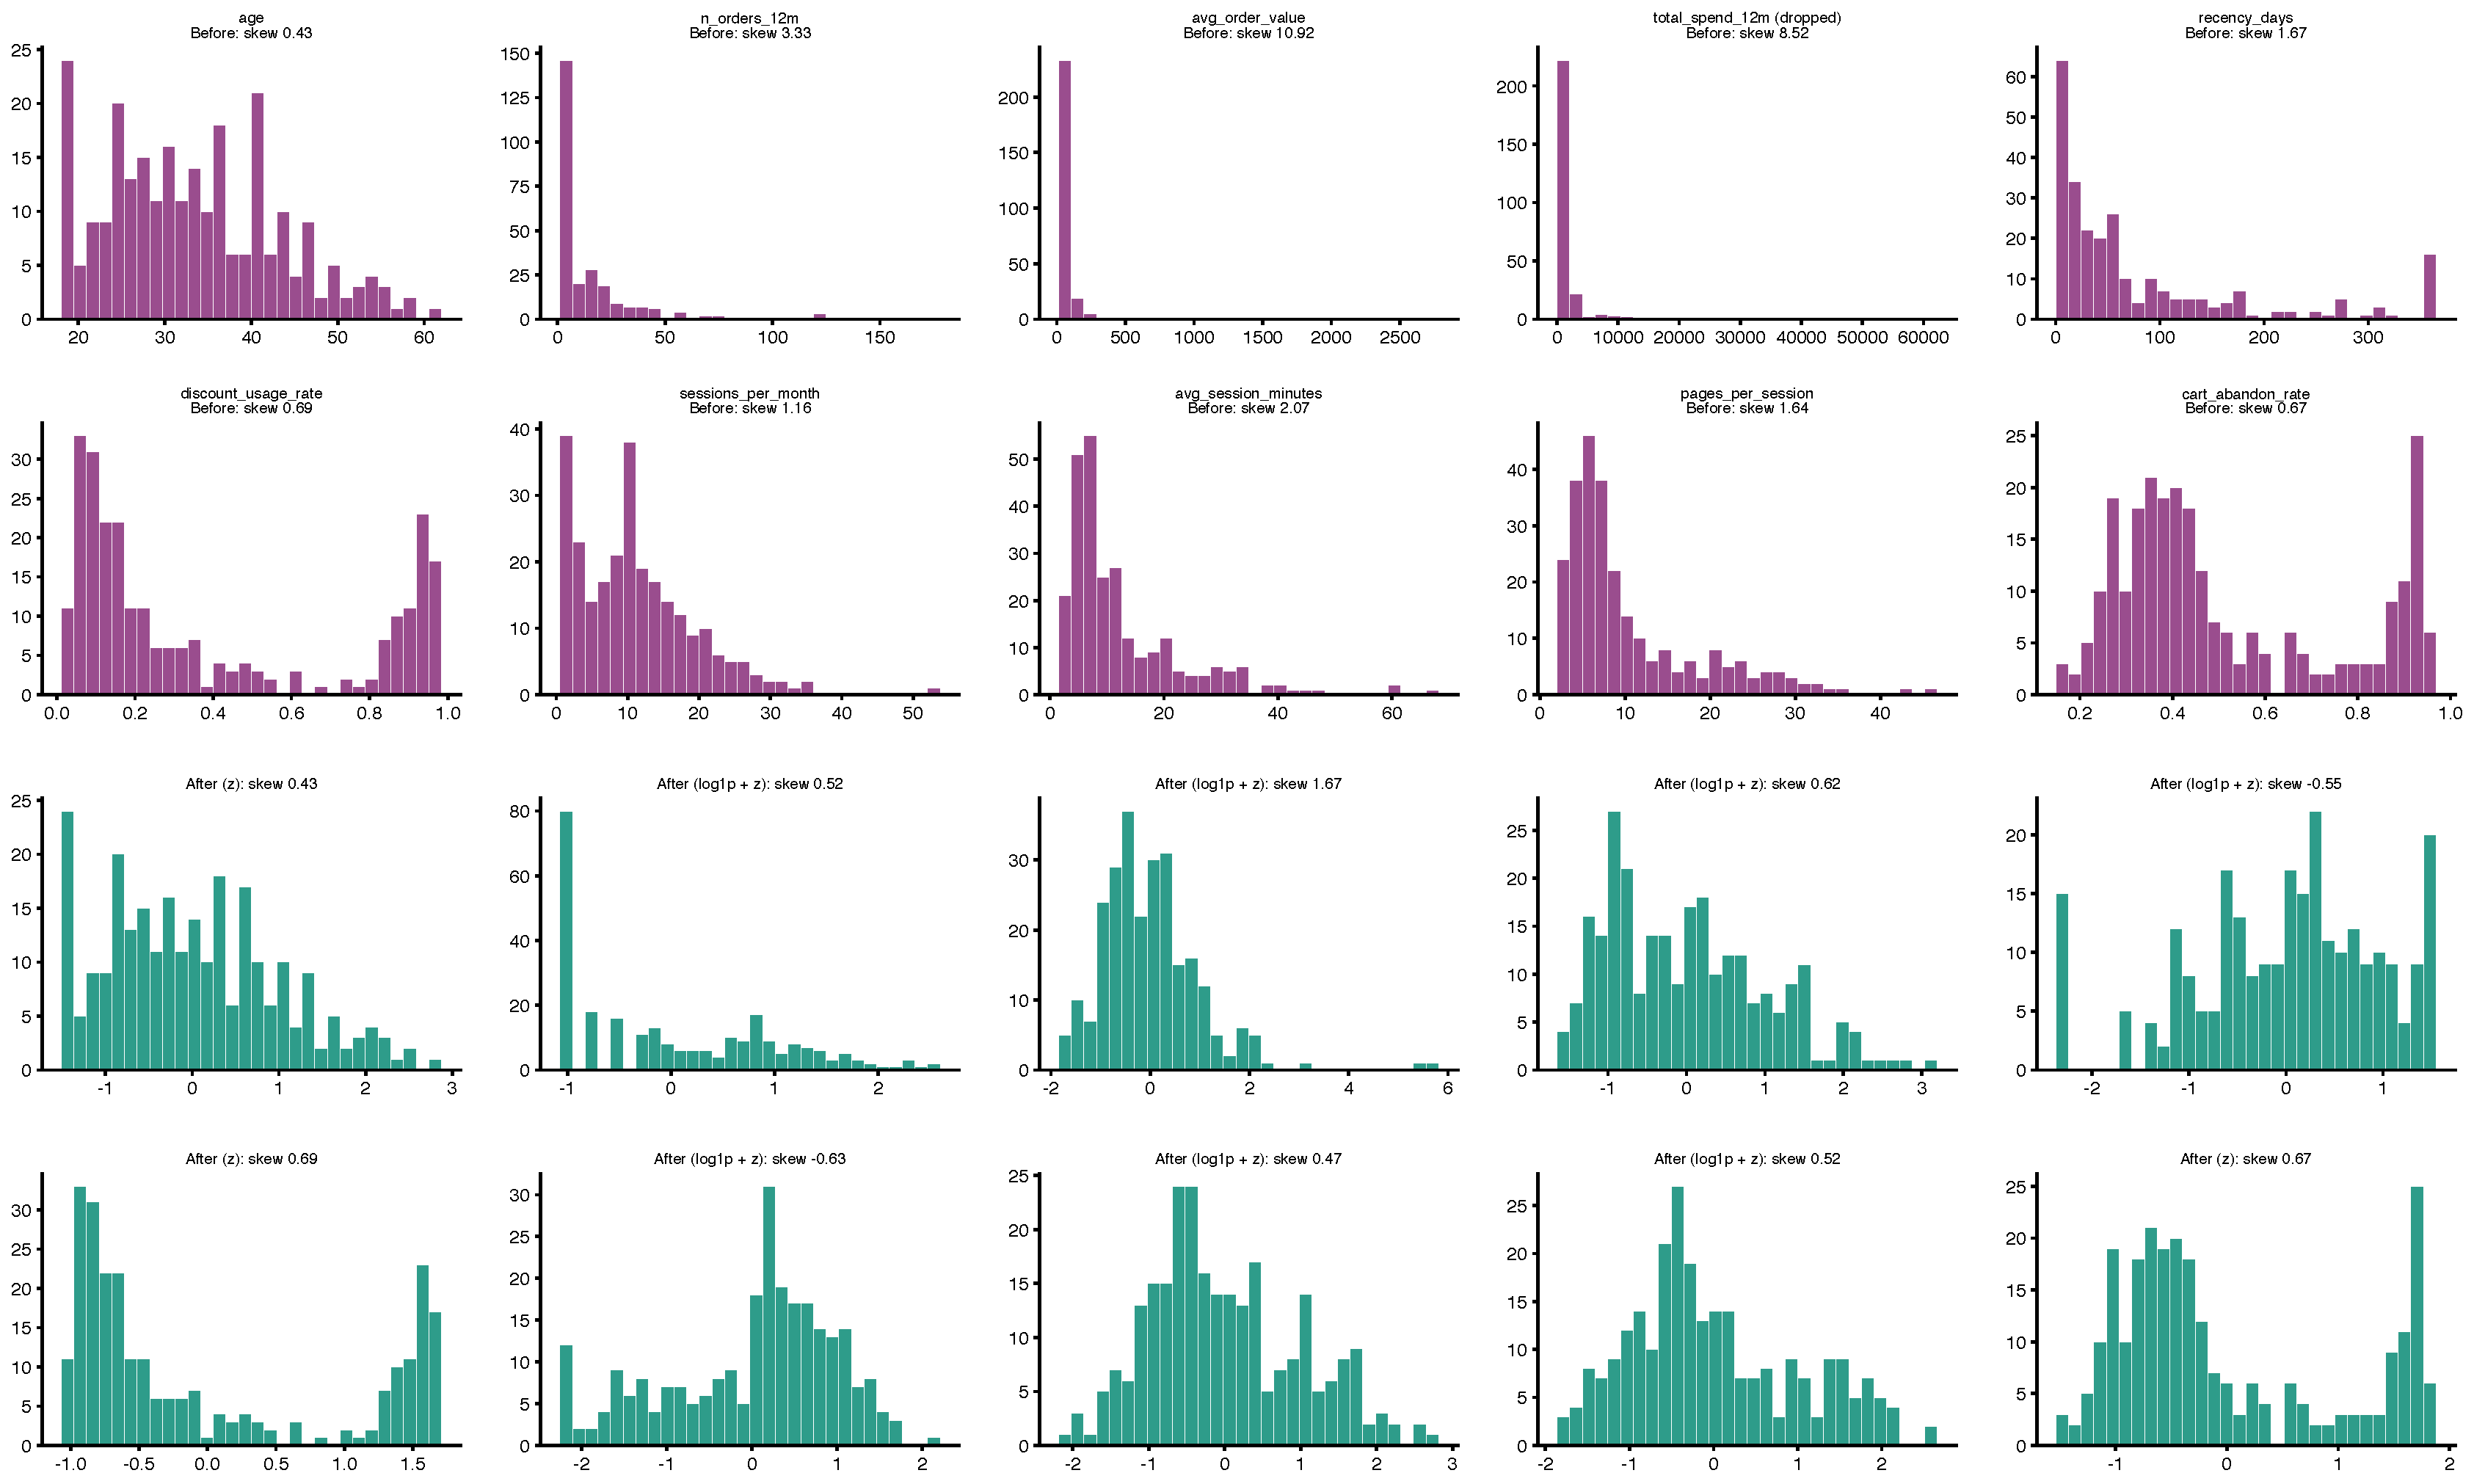
\includegraphics[width=\linewidth]{figD1_distributions_before_after.pdf}
\caption{Phân phối 10 cột số trước (hai hàng trên, tím) và sau chuẩn bị (hai hàng dưới, lam-lục). Cột \var{total_spend_12m} bị loại ở ma trận chính nhưng vẫn hiển thị. Khối cột tại $n=1$ của \var{n_orders_12m} vẫn còn sau log.}
\label{fig:d_dist}
\end{figure}

\begin{figure}[htbp]
\centering
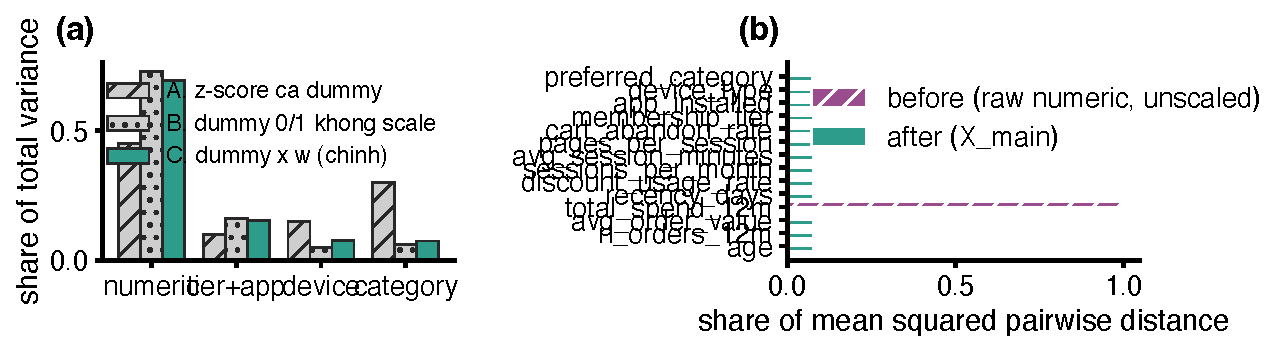
\includegraphics[width=\linewidth]{figD3_encoding_and_distance_share.pdf}
\caption{(a) Tỉ trọng phương sai theo khối với ba cách mã hóa (C là phương án chính). (b) Tỉ trọng bình phương khoảng cách theo thuộc tính gốc: trước chuẩn bị (tím, số thô không scale) và sau (lam-lục).}
\label{fig:d_enc}
\end{figure}

\begin{figure}[htbp]
\centering
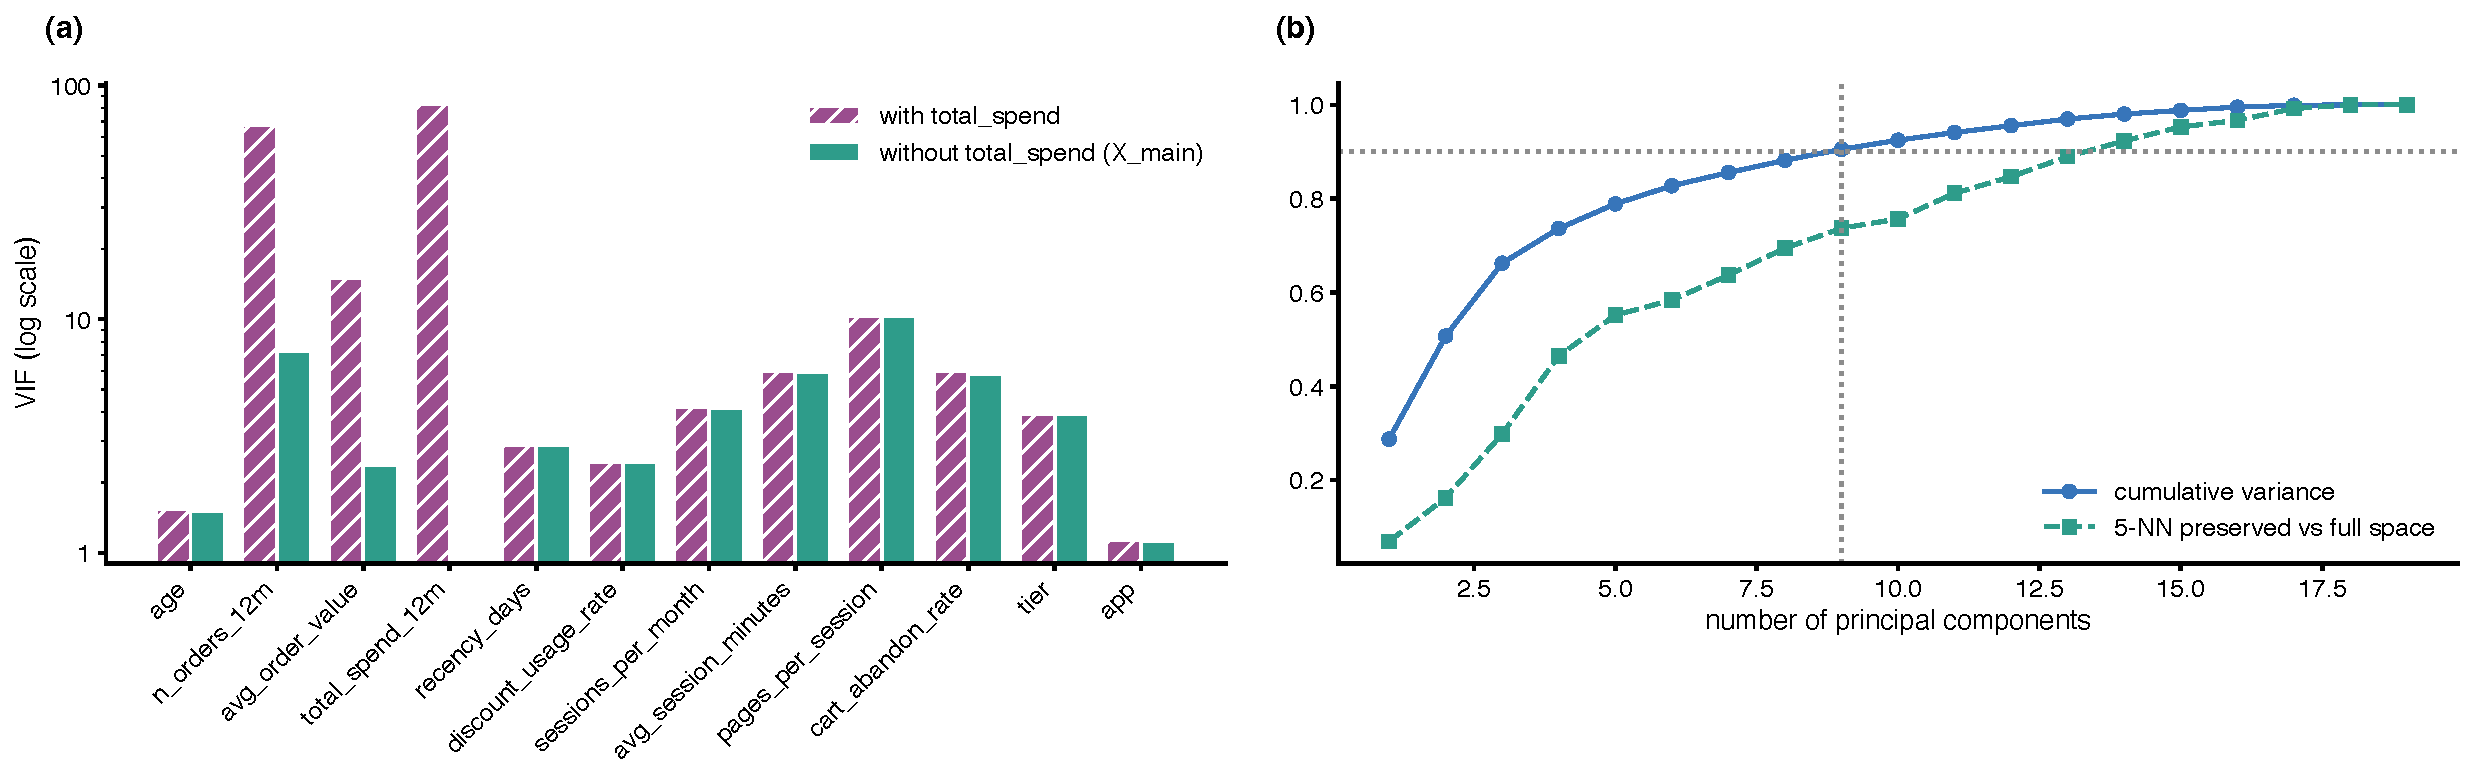
\includegraphics[width=\linewidth]{figD4_redundancy_and_pca.pdf}
\caption{(a) VIF trên thang log khi có và không có \var{total_spend_12m}. (b) Phương sai tích lũy và mức giữ lân cận 5-NN theo số thành phần PCA: 90\% phương sai (9 thành phần) chỉ giữ 74\% lân cận.}
\label{fig:d_red}
\end{figure}

\begin{table}[htbp]
\centering\small
\caption{Các phiên bản ma trận đã lưu và mức đồng thuận hình học với ma trận chính (5-NN trùng; tương quan hạng của khoảng cách cặp).}
\label{tab:variants}
\begin{tabular}{lccc}
\toprule
Phiên bản & Số cột & 5-NN trùng & Tương quan hạng\\
\midrule
\var{full_features} (còn total\_spend) & 20 & 0,939 & 0,993\\
\var{cat_unknown_col} & 20 & 0,966 & $>0{,}999$\\
\var{cat_knn7} & 19 & 0,959 & $>0{,}999$\\
\var{cat_mode} & 19 & 0,941 & $>0{,}999$\\
\var{no_category} & 14 & 0,685 & 0,997\\
\texttt{pca90} & 9 & 0,737 & 0,995\\
Gower (ma trận khoảng cách) & -- & 0,708 & 0,894\\
\bottomrule
\end{tabular}
\end{table}

Bộ biến đổi được lưu bằng sklearn (\texttt{ColumnTransformer}, \texttt{joblib}) cùng siêu dữ liệu từng cột, cấu hình và mã băm; nạp lại trong tiến trình mới tái tạo $X_{\text{main}}$ với sai khác lớn nhất $4{,}4\times10^{-16}$,
và tái dựng tay bằng NumPy cho kết quả khớp. Nghiệm thu 13/13 đạt.
\FloatBarrier
